\section{Definition}

The reactivity coefficient, denoted as $\alpha$, is defined as:
\begin{equation}
    \alpha = \frac{\partial \rho}{\partial x}
\end{equation}
where $x$ represents a certain quantity that affects the reactivity, $\rho$.

\section{Reactivity Coefficients for Different Components}

For our case, we consider the following reactivity coefficients.

\begin{itemize}
    \item $\alpha_f$ = Fuel reactivity coefficient
    \item $\alpha_m$ = Moderator reactivity coefficient
    \item $\alpha_c$ = Coolant reactivity coefficient
    \item $\alpha_e$ = Reactivity due to thermal expansion of the fuel
\end{itemize}

In the TRIGA reactor, $\alpha_e$ can often be neglected because, as in other thermal systems, the thermal expansion is smaller compared to the migration length of neutrons.

\begin{tcolorbox}[boxstyle2]
\textbf{Note for fast reactors:} The higher migration length in fast reactors makes the reactivity effect of thermal expansion more relevant.
\end{tcolorbox}

\section{Doppler Effect}

The fuel reactivity coefficient, $\alpha_f$, is primarily due to the Doppler effect. The Doppler effect causes a broadening of the resonance peaks in the absorption cross-section of the fuel.

\begin{equation}
    \sigma(\text{fuel, E}) = \text{Doppler Effect}
\end{equation}

\begin{figure}[h]
    \centering
        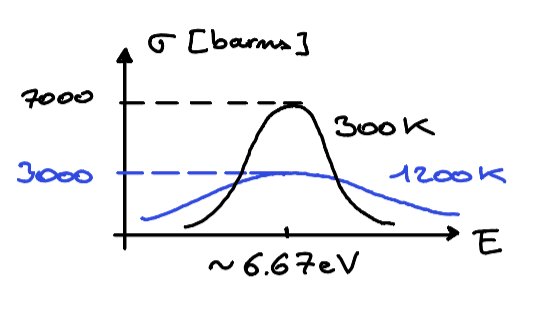
\includegraphics[width=0.75\linewidth]{doppler.png}
    \caption{The Doppler effect shows the broadening of resonance peaks.}
\end{figure}

\section{Functions of Reactivity Coefficients}

Specifically for the TRIGA reactor:
\begin{itemize}
    \item $\alpha < 0$ indicates a \textbf{negative reactivity coefficient}, which is essential for safety.
    \item $\alpha \ll 0$ allows for stable operation in \textit{pulse mode}.
\end{itemize}

\section{Design Considerations}

When designing a system with fuel and moderator, consider the following:
\begin{itemize}
    \item Increase in temperature ($T \uparrow$) leads to reduced moderation capability, affecting the neutron flux.
    \item The effect on the absorption cross-section ($\Sigma_a \downarrow$) also reduces the reactivity.
\end{itemize}

\section{Physical Background}

The physical background involves the following dynamics:
\begin{equation}
    \frac{dn}{dt} = P - A - L + S
\end{equation}
where:
\begin{itemize}
    \item $P$ denotes production, which depends on $\Sigma_f \phi$
    \item $A$ denotes absorption, proportional to $\Sigma_a \phi$
    \item $L$ denotes leakage, related to $\nabla D \phi$
    \item $S$ denotes scattering, related to $\Sigma_s \phi$
\end{itemize}

The reactivity $\rho$ can be approximated by:
\begin{equation}
    \rho \propto \frac{P - A - L}{P}
\end{equation}

\subsection{Dependence on Parameters}

The parameters affecting reactivity are:
\begin{itemize}
    \item Temperature (affects cross-section and density)
    \item Geometry (affects distribution)
    \item Fuel condition (corrosion, burnup, etc.)
\end{itemize}

\subsection{Side Note on Fast Reactors}

In fast reactors, the coefficients $\alpha_f$ and $\alpha_c$ can be greater than zero depending on the fuel composition, as is the case with molten salt reactors where fuel is mixed with the coolant.

\section{Overview of the Effects of Reactivity Coefficients}

The following plot gives an overview of how reactivity feedbacks affect power in the reactor.
\begin{figure}[H]
    \centering
        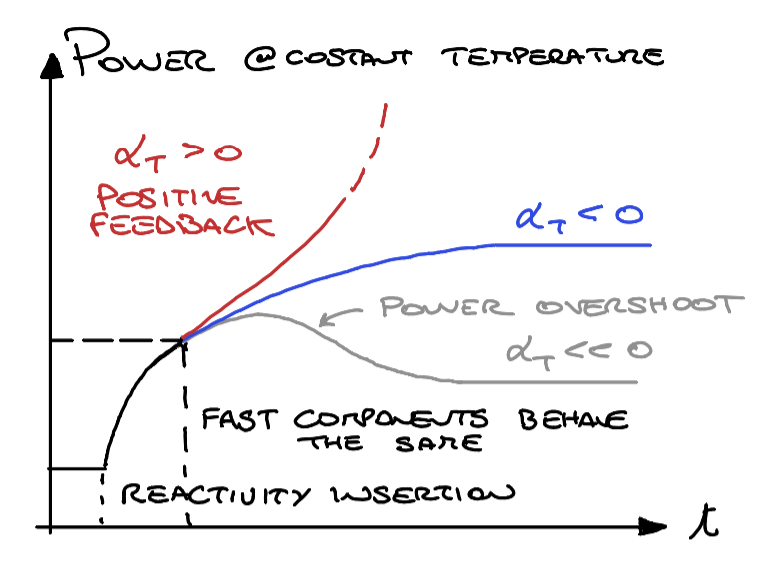
\includegraphics[width=0.6\linewidth]{power_effect.png}
    \caption{Overview of the effects of $\alpha$ on reactor power.}
\end{figure}

\section{TRIGA Fuel}

TRIGA fuel consists of Uranium-Zirconium Hydride (U-Zr-H), the solid moderator comprises hydrogen, with zirconium acting as the stabilizing element.

\subsection{Experimental Findings}

\paragraph{First Experiment: Mono-Energy Neutron Source}: Determination of the effective energy for moderation. \\
\paragraph{Second Experiment: Acoustical Resonance Study}: Influence of temperature on resonance peaks. \\
\paragraph{Third Experiment: Cross-Section Evaluation}: Measuring total removal cross-section.

\section{Explanation of the Results}

The findings from these experiments suggest that:
\begin{enumerate}
    \item Hydrogen in a lattice has no free recoil.
    \item The interference effect is characterized by a wavelength related to specific energy levels.
    \item Possibility of up-scattering due to vibration modes.
\end{enumerate}

\section{Thermalization through Bounded Nuclei}

The thermalization process occurs via two primary pathways:
\begin{enumerate}
    \item \textbf{Translation Modes}:
        \begin{itemize}
            \item Elastic interaction involving the entire crystal structure.
            \item Reduced logarithmic energy decrease with increased temperature.
        \end{itemize}
    \item \textbf{Vibration Modes}:
        \begin{itemize}
            \item Excitation of vibration states that influence up-scattering.
        \end{itemize}
    \item \textbf{Coherent and Incoherent Scattering}
\end{enumerate}

The total scattering cross-section, $\sigma_{\text{scattering}}$, consists of both coherent and incoherent components:
\begin{equation}
    \sigma_{\text{scattering}} = \sigma_{\text{coherent}} + \sigma_{\text{incoherent}}
\end{equation}
In the TRIGA reactor
\section{Elastic vs Inelastic Scattering}

Elastic scattering involves no change in the internal quantum states of the scatterer. In contrast, inelastic scattering involves changes in these states.

\begin{itemize}
    \item \textbf{Elastic}: No excitation states, such as with free hydrogen.
    \item \textbf{Inelastic}: Involves excitation related to vibrations and rotations within the molecule.
\end{itemize}

\section{Thermalization through Bounded Nuclei}

Thermalization of neutrons through bounded nuclei can occur via two primary mechanisms:
\begin{enumerate}
    \item \textbf{Translation Modes}:
        \begin{itemize}
            \item Elastic interactions that involve the entire crystal lattice.
            \item Changes in temperature lead to variations in logarithmic energy decrease.
        \end{itemize}
    \item \textbf{Vibration Modes}:
        \begin{itemize}
            \item Specific energy excitations related to vibrational modes.
            \item Absorption of vibrational energy quanta can lead to up-scattering.
        \end{itemize}
\end{enumerate}

\section{Coherent and Incoherent Scattering}

Coherent scattering occurs when scattering events result in interference effects due to the crystal structure, manifesting as Bragg peaks. Incoherent scattering, in contrast, lacks such regular interference patterns.

\begin{equation}
    \sigma_{\text{scattering}} = \sigma_{\text{coherent}} + \sigma_{\text{incoherent}}
\end{equation}

\begin{figure}[h]
    \centering
    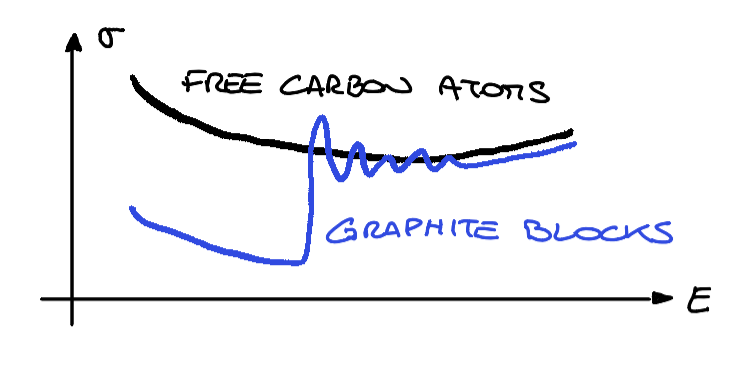
\includegraphics[width=0.75\linewidth]{coherent_vs_inchoerent.png}
    \caption{Coherent and incoherent scattering on Carbon atoms, when they form a crystalline structure in the graphite the scattering is inchoerent.}
\end{figure}

\section{Summary of Findings on TRIGA Fuel}

The experimental findings on TRIGA fuel reveal key insights into moderation and reactivity:

\begin{itemize}
    \item TRIGA fuel demonstrates effective moderation properties above a certain energy threshold.
    \item The presence of zirconium hydride contributes significantly to the observed moderation effects.
    \item Doppler effects and up-scattering play important roles in spectral hardening.
\end{itemize}

\section{Recap of Results}

To summarize, the moderation capabilities of hydrogen in zirconium hydride are influenced by several factors, including lattice structure and vibrational modes. Based on experiments and Monte Carlo simulations:

\begin{itemize}
    \item The Bragg peak is negligible in the energy range of interest.
    \item The primary mechanism involves vibrational modes related to the hydrogen lattice.
    \item Spectral hardening is observed with increasing temperature.
\end{itemize}

\begin{tcolorbox}[boxstyle2]
The findings suggest that Zr-H-based fuels exhibit complex moderation behavior, particularly at higher temperatures where vibrational modes play a significant role.
\end{tcolorbox}

\section{Additional Notes}

\subsection{Composition of fuel reactiviy coefficent in the TRIGA reactor}

A breakdown of the contributions to $\alpha_f$ in the TRIGA reactor is presented in the table below.

\begin{table}[h]
    \centering
    \begin{tabular}{|l|c|c|}
        \hline
        Contribution & Aluminum Cladding & Stainless Steel Cladding \\
        \hline
        Doppler Effect & 2.6 & 2.1 \\
        Spectral Hardening & 5.7 & 7.8 \\
        Cell Flux Effect & 3.5 & 5.7 \\
        Leakage Effect & 2.2 & 2.1 \\
        \hline
        Total $\alpha_f$ (pcm/°C) & 8.3 & 9.9 \\
        \hline
    \end{tabular}
    \caption{Breakdown of $\alpha_f$ contributions in TRIGA for different cladding materials.}
\end{table}

\subsection{TRIGA Fuel Characteristics}
TRIGA fuel (Zr-H) can moderate up to 0.13 eV and can induce upscattering, as indicated by experimental evidence, which justifies the use of H\textsubscript{2}O as a moderator.

\begin{itemize}
    \item Hydrogen is bounded to Zr, and for thermal energy, the bound cannot be neglected.
    \item Hydrogen in Zr-H moderates mainly through inelastic scattering.
    \item \textbf{Model:} Using the Einstein quantum harmonic oscillator, we can explain the experimental evidence.
\end{itemize}

In TRIGA fuel, the temperature coefficient $\alpha_T$ is approximately $-7$ to $-9$ pcm/°C.

\section{Experimental Brief}
\begin{itemize}
    \item \textbf{Step 1:} Shift out control rods $\rightarrow$ $\rho \uparrow$ $\rightarrow$ Power $\uparrow$
    \item \textbf{Step 2:} Overshoot of power is observed.
    \item \textbf{Step 3:} Compute the energy release up to the peak.
    \item \textbf{Step 4:} Estimate the temperature $T$.
    \item \textbf{Step 5:} Compute the temperature coefficient $\alpha_T$.
\end{itemize}

Note: The coolant temperature coefficient, $\alpha_{T_{\text{coolant}}}$, is slightly positive.

\section{Void Coefficient}

\subsection{Definition and Function}
The void coefficient, $\alpha_v$, is defined as:
\begin{equation}
    \alpha_v = \frac{\partial \rho}{\partial \mathcal{E}}
\end{equation}
where $\mathcal{E}$ represents the void fraction. The void coefficient plays an important role in safety, helping assess the response in situations like boiling, experiments, irradiation, and Loss of Coolant Accidents (LOCA).

\subsection{Design Considerations and Physical Background}
\begin{itemize}
    \item Changes in moderation due to void formation lead to spectral hardening, causing a decrease in the resonance escape probability $p$.
    \item Absorption decreases, increasing the thermal utilization factor $f$.
    \item Leakage increases, reducing the probability of non-leakage $P_{NL}$.
\end{itemize}

\begin{figure}[H]
    \centering
    
\includegraphics[width=0.75\linewidth]{placeholder.png}
    \caption{Effect of moderation ratio on $k_{\text{eff}}$.}
\end{figure}

\section{Impact on the Six-Factor Formula}

\begin{itemize}
    \item $p$: Resonance escape probability
    \begin{equation}
        \alpha_{p,i} = \ln \left( \frac{1}{p} \right) \left( \frac{1}{N_H V_H} \frac{\partial N_H V_H}{\partial V} \right) = \frac{\partial p}{\partial V}
    \end{equation}
    
    \item $f$: Thermal utilization factor
    \begin{equation}
        \alpha_{f,i} = (1 - f) \left( - \frac{1}{N_H V_H} \frac{\partial N_H V_H}{\partial V} \right)
    \end{equation}
\end{itemize}

These coefficients are strongly dependent on absorption and moderation capacity. For example:
\begin{itemize}
    \item \textbf{Void in Fuel} $\rightarrow \rho \downarrow$
    \item \textbf{Void in Water} $\rightarrow \rho \uparrow$
\end{itemize}

\section{Experiment Outline}
\begin{enumerate}
    \item Start at zero power, aiming to create a void.
    \item Ensure zero power, clean, and critical conditions.
    \item Register control rod positions.
    \item Insert a sample filled with water:
    \begin{itemize}
        \item If $\alpha_v < 0$, $\rho \uparrow$
    \end{itemize}
    \item Return to criticality by adjusting the control rods.
    \item Find control rod calibration curves to determine $\Delta \rho$.
\end{enumerate}

\textbf{Samples:} Placed in one of the channels.

\subsection{Examples of Void Experiments}
\begin{itemize}
    \item \textbf{In Ljubljana:} Bubbles were injected into the core. Monte Carlo simulations confirmed that $\alpha_v < 0$.
    \item \textbf{In Vienna:} Fuel elements with 70\% enrichment were used, making $\alpha_v > 0$ due to high enrichment and the limited need for moderation.
\end{itemize}

\section{Effects on Neutronics}

The reactivity $k$ can be expressed as:
\begin{equation}
    k = \eta f \epsilon P_{NL} P_{NL}
\end{equation}

The differential of $k$ with respect to a parameter $x_i$ can be expanded:
\begin{equation}
    \alpha_i = \frac{\partial \rho}{\partial x_i} = \frac{1}{k} \frac{\partial k}{\partial x_i} = \frac{1}{\eta} \frac{\partial \eta}{\partial x_i} + \frac{1}{f} \frac{\partial f}{\partial x_i} + \frac{1}{\epsilon} \frac{\partial \epsilon}{\partial x_i} + \dots
\end{equation}

\begin{itemize}
    \item \textbf{Doppler Effect:} Variations in resonance weight due to self-shielding.
    \item \textbf{Spatial Self-Shielding:} Outer rings of the fuel pin shield the center, reducing the flux at the core.
\end{itemize}

\section{Spectral Hardening}

Spectral hardening occurs due to the harmonic oscillator behavior of Zr-H:
\begin{equation}
    \alpha_{f,i} \approx \frac{1}{\Sigma_a^f} \frac{\partial \Sigma_a^f}{\partial x_i} - \frac{1}{\Sigma_a^m} \frac{\partial \Sigma_a^m}{\partial x_i} - \frac{1}{\phi} \frac{\partial \phi}{\partial x_i}
\end{equation}

In fuel, spectral hardening increases the mean free path, affecting capture and escape probabilities.

\subsection{Disadvantage Factor}
\begin{equation}
    \zeta = \frac{\phi_{\text{moderator}}}{\phi_{\text{fuel}}}
\end{equation}

Since spectral hardening is stronger in the fuel, the ratio of escaping flux from the fuel is higher.

\section{Experimental Procedure}

This procedure yields a reactivity temperature coefficient rather than a prompt fuel coefficient.

\begin{itemize}
    \item Measure $\Delta T$ due to $\Delta \rho$ and compute the ratio.
    \item No direct way to measure $T_f$ (limited thermocouples, coolant contribution).
\end{itemize}

\subsection{Simple Approach}
\begin{enumerate}
    \item Set reactor at desired power.
    \item Record control rod position and extract positive reactivity.
    \item Record power variation.
    \item Calculate energy released until peak.
    \item Calculate average temperature difference.
    \begin{equation}
        \Delta T_f = \frac{E}{G_f(N_f)}
    \end{equation}
    \item Calculate the $\beta$ temperature coefficient.
\end{enumerate}

\section{Coolant Effects}

\subsection{Components}
Two contributions:
\begin{itemize}
    \item Water density decrease, leading to $\rho \downarrow$
    \item Different rod capacity of H in water, leading to $\rho \uparrow$
\end{itemize}

Overall, $\alpha_{T_{\text{coolant}}} < 0$, although some contributions can be positive.

\subsection{Isothermal Coefficient}
\begin{equation}
    \alpha_{\text{iso}} = \alpha_{T_f} + \alpha_{T_c}
\end{equation}
Observed in Ljubljana by changing pool conditions while maintaining core conditions.

\begin{equation}
    \alpha_{\text{iso}} = -3 + 6.5 = +3.5 \text{ pcm/°C}
\end{equation}

\textbf{Experimental Note:} Despite positive contributions, $\alpha_{T_c} < 0$ overall.
